\chapter{Methodik}

TODO

%%%%%

\section{Untersuchungsdesign}

% Verfahrensteckbrief me

\begin{table}[H]
    \centering
    \begin{tabular}{>{\raggedright\arraybackslash}p{0.2\linewidth}>{\raggedright\arraybackslash}p{0.75\linewidth}}\toprule\toprule
         \textbf{Verfahren}& Syntaktisches Similarity Hashing\\\hline\hline
         \textbf{Untersuchungsziele}& SCI (Unterscheidung nativer Kameraaufnahmen und KI-generierter Videos) und SNA (Erkennung komprimierter Social-Media-Videos)\\\hline
         \textbf{Feature}& Extrahierte 4CC-Box-Informationen unter Ausschluss der Inhaltsdaten (\(mdat\)) und volatile Metadaten (z. B. Zeitstempel wie \(creationTime\))\\\hline
         \textbf{Symbolische Repräsentation} (T1 bis T5)& TODO: linearisiert die in JSON erfasste hierarchische Baumstruktur in eindimensionale Token-Sequenzen, ohne vertikale Pfade zu extrahieren\\\hline
         \textbf{Feature-Repräsentation}& n-Gramm-Sets (Similarity Digest)\\\hline
         \textbf{Feature-Selektion}& Allowlisting relevanter Container-Boxen und Dubletteneliminierung\\\hline
         \textbf{Klassifikator}& Approximate Matching (Ähnlichkeitsberechnung mittels Jaccard-Index oder asymmetrischem Tversky-Index)\\\hline
         \textbf{Datenbanken}& VISION, EVA-7K und ein eigens erstellter Datensatz zu KI-generierten Videos\\\hline
         \textbf{Test- und Trainingsdaten}& Bildung von Referenz-Hashes (Source Similarity Digests) aus einer kleinen, diversen Teilmenge (z. B. ein Bild pro Aufnahmemodus), Abgleich mit allen restlichen Testdateien\\\hline
         \textbf{Evaluation}&Native Aufnahmen, Social Media, synthetische Inhalte und gemischte Inhalte\\\hline
         \textbf{Metriken}&Receiver Operating Characteristic (ROC) und Area Under Curve (AUC)\\ \bottomrule\bottomrule
    \end{tabular}
    \caption{Verfahrenssteckbrief zum Similartiy Hashing für Mp4-Dateien (Eigene Darstellung)}
    \label{tab:steckbrief-mp4}
\end{table}

%%%%%

\newpage
\section{Vorgehen und Datenpipeline}

TODO

\subsection{Vorgehen}

TODO: Stichpunkte ausformulieren

% Grafik des Vorgehens

\begin{figure}[H]
    \centering
    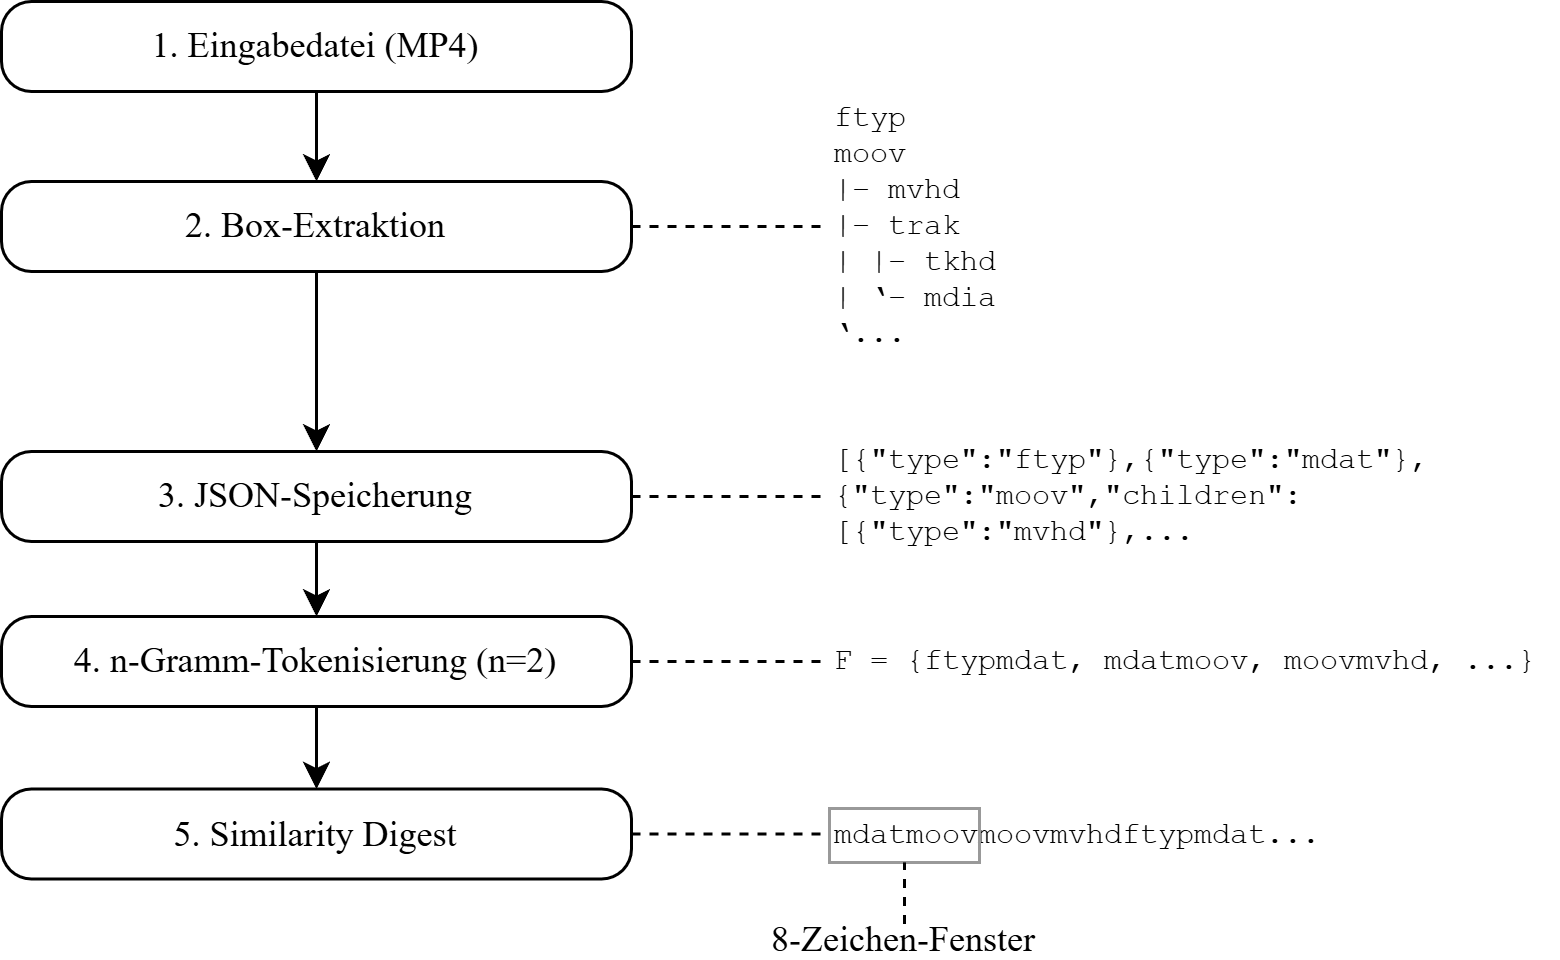
\includegraphics[width=1\linewidth]{grafiken/vorgehen-mp4.drawio.png}
    \caption{TODO: vorgehen-mp4.drawio.png}
    \label{fig:vorgehen}
\end{figure}

% Stichpunkte Vorgehen

\begin{enumerate}
    \item Mp4 Dateien parsen
    \item Box-Informationen extrahieren
    \item Box-Struktur im JSON-Format abspeichern
    \item Box-Struktur linearisieren und als 2-Gramme tokenisieren
    \item 2-Gramme als Similarity Digest abspeichern und die mit 8-Zeichen-Fenster auslesbar sind
\end{enumerate}

%%%

\newpage
\subsection{Datenpipeline}

TODO: Stichpunkte ausformulieren

% BPMN der Pipeline

\begin{figure}[H]
    \centering
    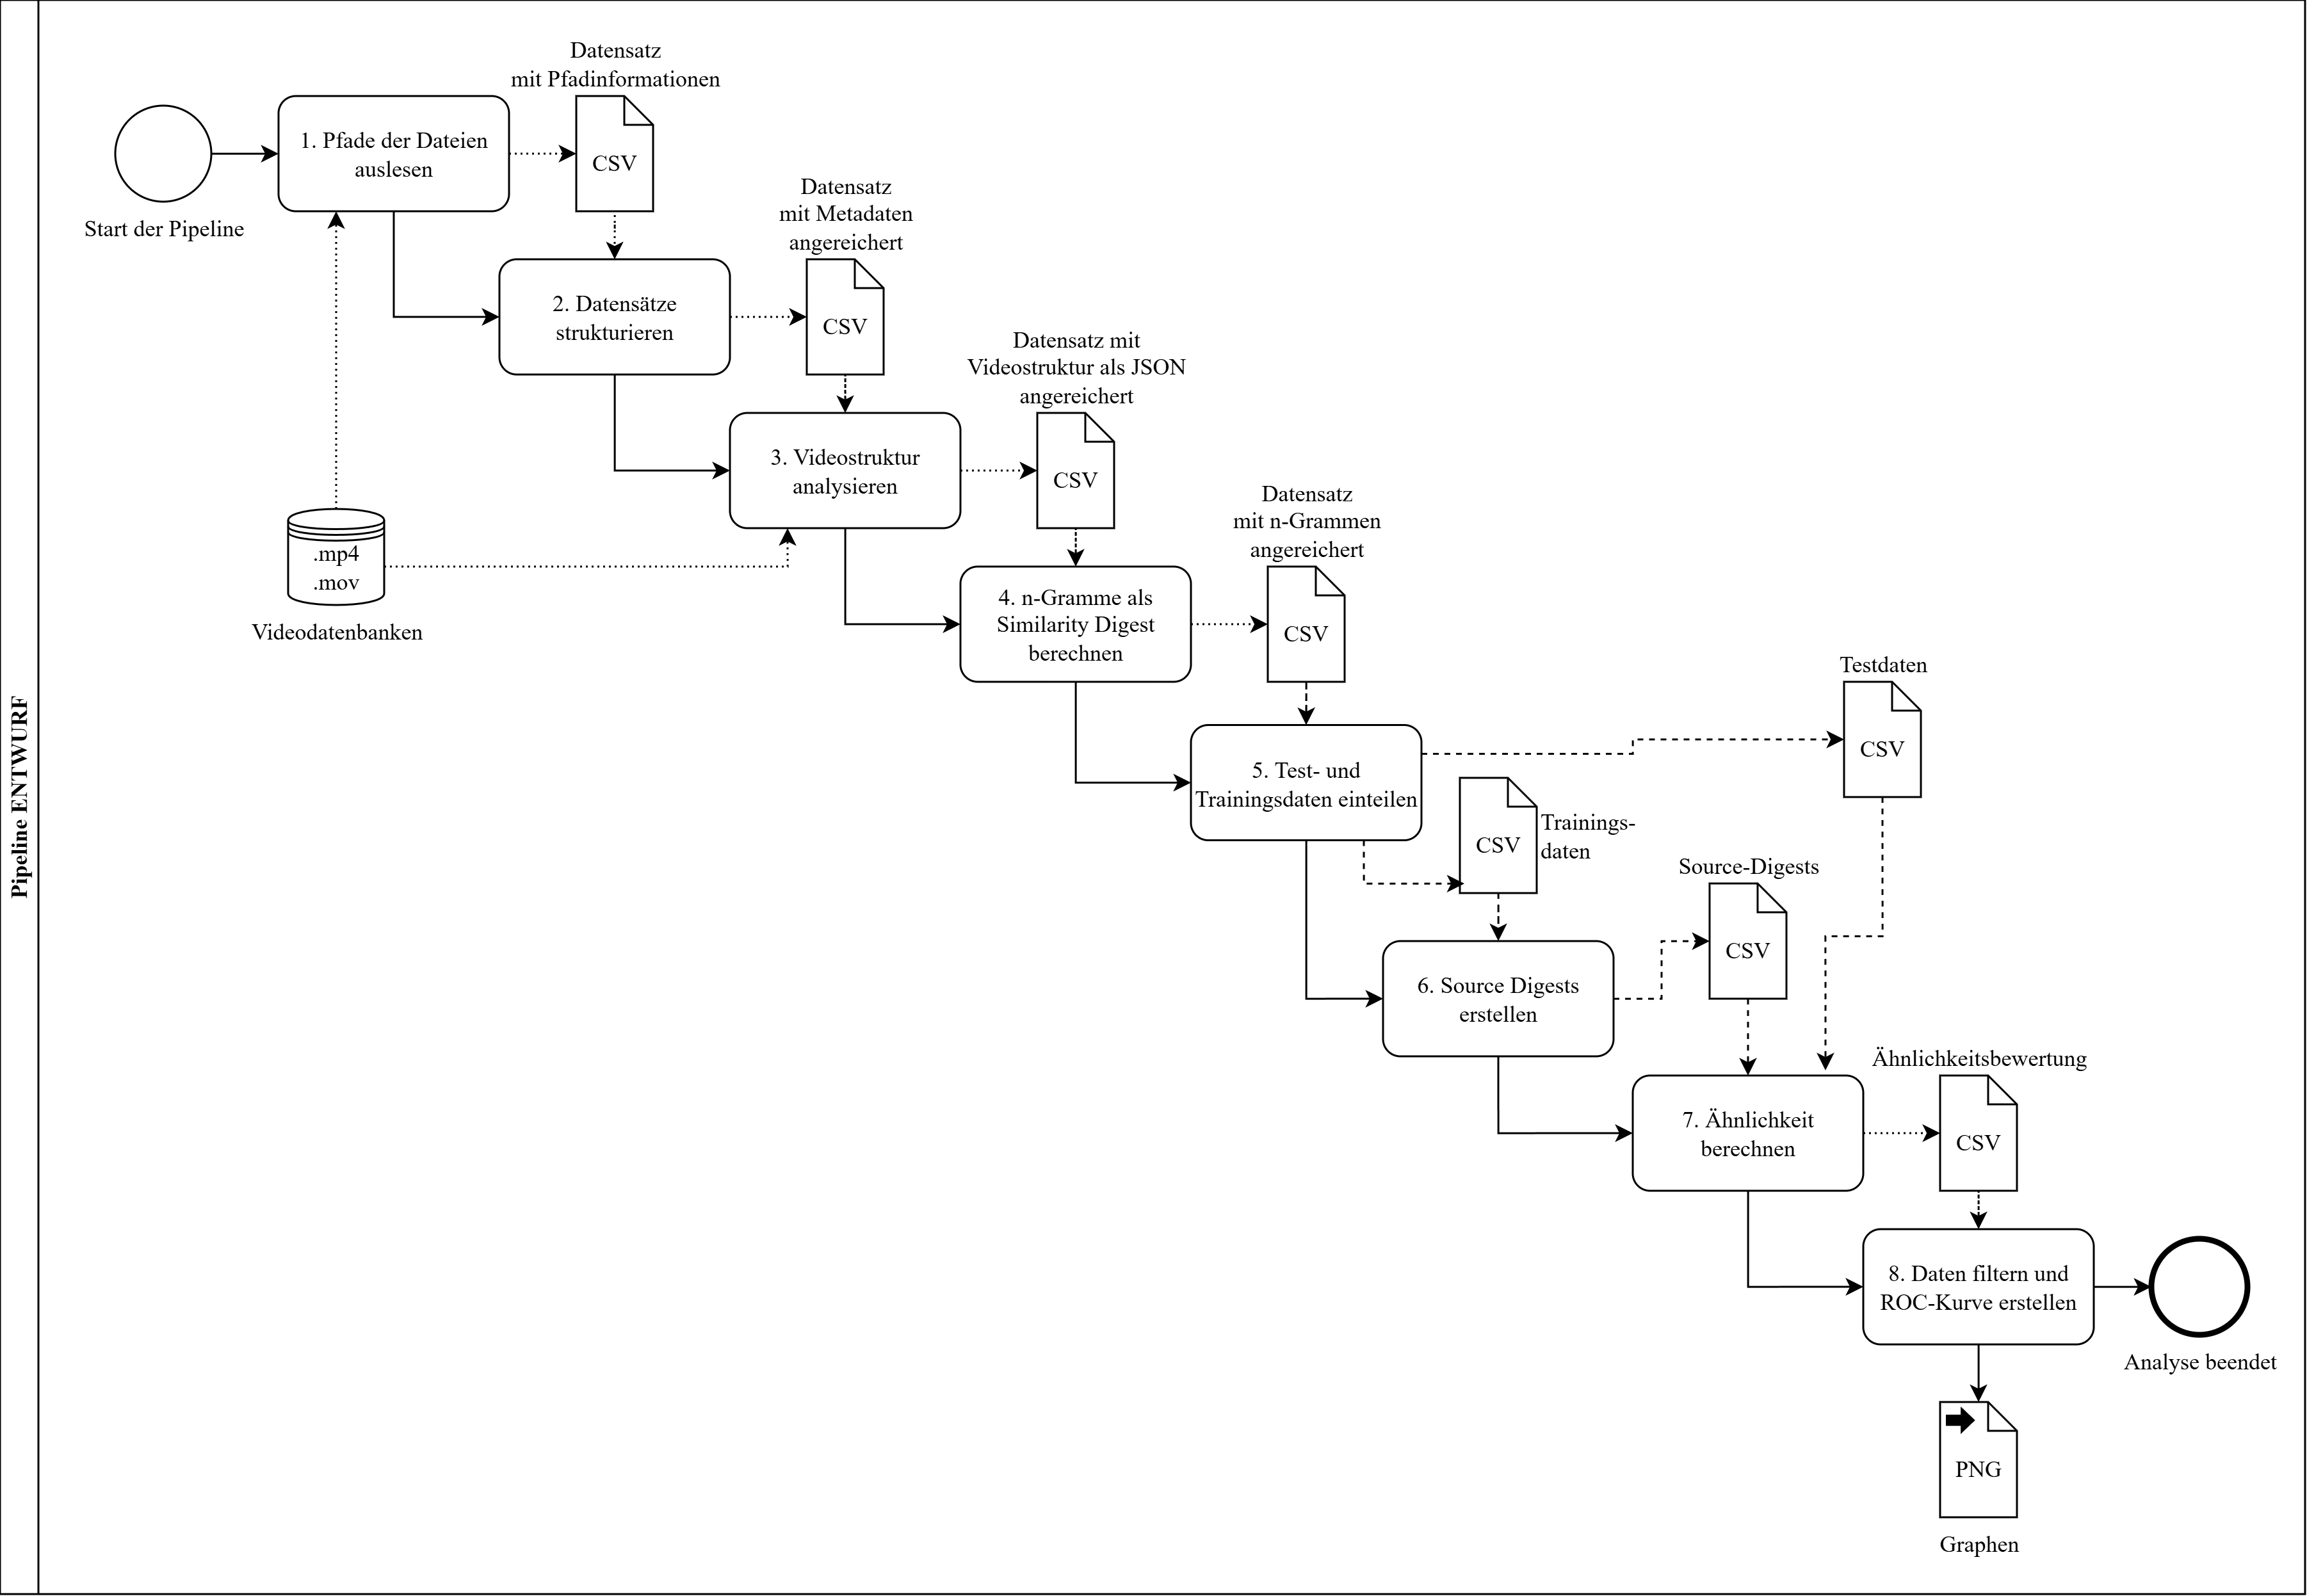
\includegraphics[width=1\linewidth]{grafiken/pipeline.drawio.png}
    \caption{TODO: pipeline.drawio.png}
    \label{fig:pipeline}
\end{figure}

% Stichpunkte Pipeline

\begin{enumerate}
    \setcounter{enumi}{-1}
    \item \textbf{Videodatenbanken bereitstellen}
    \begin{itemize}
        \item EVA-7k (5.684 Dateien)
        \item VISION (nur Videos, 1918 Dateien)
        \item eigener KI-Datensatz
    \end{itemize}
    
    \item \textbf{Pfad jeder einzelnen Videodatei auslesen}
    \begin{itemize}
        \item PATH (Dateipfad z.\,B. \url{C:/Testdaten/EVA/D01_flat_yt.mp4})
    \end{itemize}
    
    \item \textbf{Datensätze strukturieren}
    \begin{itemize}
        \item DB\_NAME (Name der Datenbank z.\,B. Vision, Eva, Selfmade)
        \item ID (Eindeutige Kennung des Geräts (\textit{Device} bei Eva/Vision) oder der AI z.\,B. D01, AI01)
        \item BRAND (Hersteller des Smartphones oder der KI z.\,B. Samsung, Grok)
        \item MODEL (Genaue Version des Smartphones oder der KI z.\,B. GalaxyS3Mini, Imagine\_0.9)
        \item MEDIA\_TYPE (Dateiendung bzw. Containerformat z.\,B. MP4, MOV)
        \item CONTENT\_SOURCE (Originäre Quelle der Videodatei, um zwischen Kameras, vollständig KI-generierten Videos mittels Text-to-Video oder Videos, die auf Bild-Vorlagen basieren (Image-to-Video), zu unterscheiden z.\,B. DIGITAL\_CAMERA, AI\_GENERATION, MIXED)
        \item CONTENT\_TYPE (Kontext der Aufnahme z.\,B. flat, indoor, outdoor, deepfake, synthetic)
        \item PROCESSING (Primäre Verarbeitung des Videos z.\,B. native, youtube, whatsapp, ai)
        \item TAMPERING (Nachträgliche Veränderung des Videos (nur Eva-DB) z.\,B. None, Avidemux)
    \end{itemize}
    
    \item \textbf{Videostruktur analysieren}
    \begin{itemize}
        \item STRUCTURE\_PRETTY (Gut lesbarer String der MP4-Struktur (nur nice to have bzw. zum Debugging) z.\,B. \texttt{moov(mvhd,trak(tkhd))})
        \item STRUCTURE\_JSON (Exakte Baumstruktur als JSON-String, der zur N-Gram-Generierung genutzt wird z.\,B. \verb|[{"type":"moov","children":[{"type":"mvhd"}]}]|)
    \end{itemize}
    
    \item \textbf{$n$-Gramme als Similarity Digest berechnen}
    \begin{itemize}
        \item NGRAM\_2 (Kompakter Similarity Digest (String), der die Signatur des Videos auf Basis von 2-Grammen (alphabetisch, duplikatbereinigt) repräsentiert; jeweils 8 lückenlose Zeichen entsprechen einem 2-Gramm-Feature z.\,B. moovmvhdtrakmvhdtraktkhd)
    \end{itemize}
    
    \item \textbf{Datensätze in Test- und Trainingsdaten einteilen}
    \begin{itemize}
        \item EVA-7k: immer die erste Datei jedes Subsets (avidemux, exiftool, \dots) aus jeder Social-Media-Kategorie (Facebook, TikTok, YouTube, \dots)
        \item VISION: immer die erste Datei jedes Content- (flat, indoor, \dots) und Processing-Types (Original, Facebook, \dots) aus jedem Device
        \item eigener KI-Datensatz: immer die erste Datei jedes KI-Modells
    \end{itemize}
    
    \item \textbf{Source-Digest erstellen}
    \begin{itemize}
        \item Digest für jede Kategorie anhand der Testdaten generieren, z.\,B. gruppiert nach Brand, Device, Social-Media, KI, KI-Modell
        \item SOURCE\_DIGEST (aggregierter Similarity Digest)
    \end{itemize}
    
    \item \textbf{Ähnlichkeit berechnen}
    \begin{itemize}
        \item GROUND\_TRUTH\_SOURCE\_DIGEST: Bezeichner für die Ground Truth, anhand der die Testdaten erstellt wurden
        \item GROUND\_TRUTH\_MP4: Bezeichner für die Ground Truth der einzelnen Test-MP4
        \item SIMILARITY: Wert von 0 bis 1 gem. Tversky-Berechnung (kein Penalty bei fehlenden Boxen in Testdatei, Penalty bei zusätzlichen Boxen in Testdatei)
    \end{itemize}
    
    \item \textbf{Daten filtern und auswerten}
    \begin{itemize}
        \item ROC und AUC berechnen
        \item Graphen erstellen
    \end{itemize}
\end{enumerate}

\begin{table}[htbp]
    \centering
    \resizebox{\textwidth}{!}{%
    \begin{tabular}{lllllllllll}
        \toprule
        \textbf{DB\_NAME} & \textbf{ID} & \textbf{BRAND} & \textbf{MODEL} & \textbf{MEDIA\_TYPE} & \textbf{CONTENT\_SOURCE} & \textbf{CONTENT\_TYPE} & \textbf{PROCESSING} & \textbf{TAMPERING} & \textbf{STRUCTURE\_PRETTY} & \textbf{NGRAM\_2 (Auszug)} \\
        \midrule
        VISION & D15 & Apple & iPhone 6 & MOV & DIGITAL\_CAMERA & FLAT & NATIVE & NONE & \texttt{moov(mvhd,trak(tkhd))} & \texttt{moovmvhdtraktkhd} \\
        EVA-7K & D01 & Samsung & GalaxyS3Mini & MP4 & DIGITAL\_CAMERA & INDOOR & YOUTUBE & AVIDEMUX & \texttt{ftypmoov(mvhd)} & \texttt{ftypmoovmoovmvhd} \\
        SELFMADE & AI01 & Grok & Imagine\_0.9 & MP4 & AI\_GENERATION & SYNTHETIC & AI & NONE & \texttt{ftypuuidmoov(mvhd)} & \texttt{ftypuuiduuidmoov} \\
        \bottomrule
    \end{tabular}%
    }
    \caption{TODO: Beispieldatensätze}
    \label{tab:testdaten_auszug}
\end{table}

TODO: Tabelle mit Auszug der echten Datensätze
% Siehe Anhang Test mit input testdatensätze.tex


%%%%%

\newpage
\section{Feature-Engineering für MP4}

TODO: Stichpunkte ausformulieren

\begin{itemize}
    \item Unterscheidung der Atome in Container und Leafs
    \item Container enthalten weitere Boxen/Atome
    \item Leafs nur Inhaltsdaten
    \item Videoinhaltsdaten (in mdat) werden nicht in der Tiefe betrachtet
    \item Valide Boxen (Container) werden als Feste Liste definiert (Allowlisting) und tiefer betrachtet
    \item Boxen außerhalb des Allowlistings werden als Blätter/Leafes behandelt und gesammelt (z. B. mvhd, stsz, uuid) da diese Hersteller-spezifisch sein können
    \item Feature-Engineering basiert auf der Prämisse des \textit{Multimedia Syntactic Similarity Hashing} (MSSH) nach Klier \& Baier \cite{klier_media_2025}
    \item Dateigrammatik des ISO Base Media File Formats (ISOBMFF) wird als digitaler Fingerabdruck der Erzeugersoftware verstanden 
\end{itemize}


\subsection{Exklusion der Inhaltsdaten}
\begin{itemize}
    \item Um inhaltliche Unabhängigkeit zu gewährleisten, werden Boxen mit Video- und Ton-Daten ausgeschlossen
    \item mdat-Container beanspruchen in der Regel 95 Prozent der Dateigröße enthalten jedoch keinerlei ISO-konforme Unteratome
\end{itemize}


\subsection{Container-Allowlist und Berücksichtigung von Legacy-Spezifikationen}

\begin{itemize}
    \item MP4-Format erlaubt theoretisch unendlich viele proprietäre Boxen
    \item Allowlist als methodischer Filter, welche Container relevante Untercontainer enthalten
    \item Berücksichtigung von historisch gewachsenen Spezifikationen und Boxen (Legacy Types) 
    \item Basis Standard ISO/IEC 14496-12: \textbf{moov, trak, mdia, minf, stbl, udta, meta, edts, dinf, stsd, mvex, moof, traf, mfra} \cite{iso_14496-12_2022}
    \item Codec-Erweiterungen ISO/IEC 14496-14 und -15 : \textbf{mp4a, avc1, hev1} \cite{iso_14496-14_2020}\cite{iso_14496-15_2024}
    \item Legacy aus Apple-Quick-Time-Zeiten: \textbf{gmhd, clip, matt, wave}\cite{apple_quicktime_2001}
    \item Siehe \cref{tab:mp4allowlisting}
\end{itemize}

\begin{table}[h]
    \centering
\caption{Valide MP4-Container gem. ISO/IEC 14496-12, -14, -15 und Apple Quick Time Legacy}
\label{tab:mp4allowlisting}
    \begin{tabular}{|l|p{2.5cm}|p{5.5cm}|p{5.5cm}|}\hline
         \textbf{Typ (4CC)}&  \textbf{Bezeichnung}&\textbf{Kurzbeschreibung}&\textbf{Besonderheiten}
\\\hline
         moov&  Movie Box&Haupt-Container für alle Metadaten des Videos& keine\\\hline
         trak&  Track Box&Einzelne Medienspur (Video, Audio oder Daten).& keine\\\hline
         mdia&  Media Box&Informationen über die Medienformate innerhalb eines Tracks& keine\\\hline
         minf&  Media Information&Container für Handler-spezifische Informationen& keine\\\hline
         stbl&  Sample Table&Zeitstempel, Größen und Offsets& keine\\\hline
         udta&  User Data&Benutzerdefinierte Metadaten (oft Hersteller-Tags)& keine\\\hline
         meta&  Metadata&Moderne Metadaten-Strukturen (z. B. C2PA oder EXIF).& Zweideutige Struktur, die in der ISO-Norm und in Apple-Legacy unterschiedlich spezifiziert sind\\\hline
         edts&  Edit Box&Definiert Abspiel-Modifikationen (z. B. Audio-Offsets).& keine\\\hline
         dinf&  Data Information&Verweist auf den Ort der eigentlichen Mediendaten& keine\\\hline
 stsd& Sample Description&Container für Codec-spezifische Konfigurationsdetails& Definierte sog. FullBox und besitzt erweiterte Header-Daten\\\hline
 avc1& H.264 Entry&Parameter des H.264 Videocodecs&Beinhaltet massive binäre Parameter, welche die Baumstruktur unterbrechen und gesondert behandelt werden müssen\\\hline
 hev1& HEVC Entry&Parameter des H.265 (HEVC) Videocodecs&Beinhaltet massive binäre Parameter, welche die Baumstruktur unterbrechen und gesondert behandelt werden müssen\\\hline
 mp4a& Audio Entry&Container für Audio-Codec-Einstellungen (z. B. AAC).&Beinhaltet massive binäre Parameter, welche die Baumstruktur unterbrechen und gesondert behandelt werden müssen\\\hline
 wave& QuickTime Audio&Alte Audio-Eigenschaften (Legacy)& keine\\\hline
 mvex& Movie Extends&Kennzeichnet die Nutzung von Fragmented MP4 (Streaming).& keine\\\hline
 moof& Movie Fragment&Metadaten für einzelnes Video-Fragment& keine\\\hline
 traf& Track Fragment&Informationen innerhalb eines Movie Fragments& keine\\\hline
 mfra& Movie Fragment Random Access&Index für den schnellen Zugriff auf Fragmente& keine\\\hline
 gmhd& Generic Media Header&QuickTime-Container für allgemeine Medieninfos (Legacy)& keine\\\hline
 clip& Clipping Box&Bestimmt den sichtbaren Bereich des Videos (Legacy)& keine\\\hline
 matt& Track Matte Box&Definiert Masken für die Videospur (Legacy).& keine\\ \hline
    \end{tabular}
\end{table}

\subsection{Leafs}
\begin{itemize}
    \item Im Kontext synthetischer Medien sind bestimmte Atome besonders relevant
    \item Auftreten, Größe und Position der uuid-Box (von ISO als Blanko-Container erfunden) dient als primärer Herkunftsnachweis 
    \item Nutzung uuid durch die Coalition for Content Provenance and Authenticity (C2PA) standardisiert 
    \item Integration kryptografischer Metadaten-Manifeste führt bei serverseitigen KI-Muxern häufig zu massiven uuid-Blöcken am Dateianfang 
    \item Inhalt als auch Auslesen der 16-Byte-Signatur der uuid ist bei syntaktischer Auswertung irrelevant, Inhalt bleibt unbetrachtete Blackbox
\end{itemize}

\subsection{Transformation}

\begin{itemize}
    \item Überführung des n-dimensionalen MP4-Baumes in ein eindimensionales, serialisiertes Format 
    \item Topologie  durch feste Syntaxregeln
    \item Top-Level-Atome werden  verkettet und Verschachtelungen (z. B. Track-Struktur innerhalb moov) durch Klammern abgebildet
    \item Resultat: Kompakter Struktur-String zur Verwendung von n-Grammen
\end{itemize}

\section{Ähnlichkeitsanalyse}

\begin{itemize}
    \item Buzzwords: Feature Sets, Similarity Digest, Similarity Calculation
    \item Zerlegung der sequenziellen Atom-Kette in diskrete Token, wobei jedes 4-Byte-Atom als eigenständiges Merkmal behandelt wird 
    \item Sliding-Window-Verfahren überführt Token-Sequenz in n-Gramme unterschiedlicher Längen, um lokale Nachbarschaften abzubilden
    \item Mengen an n-Grammen bilden den Similarity Digest, der als kompakter, mathematisch handhabbarer Fingerabdruck der ursprünglichen Datei fungiert 
    \item Wahl der Vergleichsmetrik  (TODO)
\end{itemize}



%%%%%



\section{Implementierung des Prototyps}

https://github.com/lmechelk/mp4-structure-hash

\subsection{Parse}

\begin{itemize}
    \item Umsetzung der Feature-Extraktion erfolgt durch Python-basierten Parser, dessen grundlegende I/O-Architektur auf dem Open-Source-Skript mp4atoms.py von Emanuele Ruffaldi aufbaut \cite{emanuele_ruffaldi_dump_2024}
    \item Speichereffizientes Lesen der einzelnen Box-Header wird dabei unverändert über Memory Mapping (mmap) realisiert
    \item Steuerung über Allowlist, in die der Parser rekursiv absteigen darf
    \item Payload wird explizit von der Erfassung ausgeschlossen und Beachtung der "Large Box" bei riesigen Videodateien \cite[Kap. 4.2]{iso_14496-12_2022}
    \item Auslesen der 8-Byte Header (enthält Box-Größe und 4CC)
    \item Implementierung einer dynamischen Offset-Korrektur gem. \cref{tab:mp4ausnahmeboxen} zur fehlerfreien Traversierung normativer Ausnahmen im ISO-Standard, sog. "Full Box" (Sonderbehandlung für diese Boxen: meta, stsd, avc1, hev1, mp4a)
    \item Ausgelesene Baumstruktur wird aggregiert und als eindimensionalen String exportiert, der aber weiterhin Informationen zur Topologie enthält
    \item Beispiel String-Format: moov(mvhd,trak(tkhd))
    \item Struktur wird also in ein Format überführt, das den theoretischen Anforderungen des Syntactic Similarity Hashing (vgl. Klier \& Baier\cite{klier_github_2025}) für den maschinellen Vergleich gerecht wird
\end{itemize}

\begin{table}[h]
    \centering
\caption{Ausnahmeregelungen und Offset-Korrekturen beim Parsing}
\label{tab:mp4ausnahmeboxen}
    \begin{tabular}{|l|p{4.5cm}|p{6.5cm}|}\hline
         \textbf{Typ (4CC)} & \textbf{Strukturelle Abweichung im Binärstrom} & \textbf{Implementierte Lösungslogik (Offset-Korrektur)} \\\hline
         meta & Spezifikationskonflikt zwischen Apple-Legacy (Standard-Container) und neuer ISO-Norm (FullBox mit Versions- und Flag-Bytes) & Vorschau der ersten 4 Bytes und bei Detektion von Null-Bytes (\texttt{0x00000000}) erfolgt ein Offset-Sprung von +4 Bytes, andernfalls +0 Bytes \\\hline
         stsd & Container ist als FullBox deklariert und erzwingt im Anschluss einen zusätzlichen 32-Bit-Zähler & Start-Offset für den rekursiven Abstieg in die Unterboxen wird fix um +8 Bytes verschoben \\\hline
         avc1, hev1 & Visuelle Sample Entries und weisen direkt nach dem Header zwingend 78 Bytes an binären Bildparametern auf, bevor Unterboxen beginnen & Überspringen der binären Videodaten durch eine Offset-Verschiebung von +78 Bytes\\\hline
         mp4a & Auditiver Sample Entry und weist nach dem Standard-Header zwingend 28 Bytes an binären Audioparametern auf & Überspringen der binären Audiodaten durch eine Offset-Verschiebung von +28 Bytes\\\hline
    \end{tabular}
\end{table}

\subsection{Compare}

\begin{itemize}
    \item Klasse \verb|Mp4StructureDigest| übernimmt die Bereinigung des Struktur-Strings von sämtlichen syntaktischen Separatoren (Klammern, Pipes)
    \item Speicherung als Liste durch Slicing als 4-Zeichen-Blöcke
    \item Generierung der n-Gramme erfolgt über eine Methode, welche die Atome zu unveränderlichen Tuples zusammenfasst und Dubletten durch die Überführung in Python-Sets eliminiert.
    \item Klasse \verb|SimilarityCalculator| führt die mathematischen Mengenoperationen durch 
\end{itemize}



%%%%%



\section{Eigener KI-Video-Datensatz}

\begin{itemize}
    \item Auswahl der Generatoren
    \item Vorgehen der Erstellung von Testvideos
    \item Text-Prompts und Bildvorlagen
    \item Link auf Datensatz
    \item Generative KI-Modelle können bereits jetzt fotorealistische Videos anhand von Text oder Deepfakes mittels Bildmaterial generieren und überwiegend im MP4-Containerformat ausgeben (siehe Table 2)
    \item z. B. Imagine 0.9 von xAI das über die Plattform Grok angeboten wird
\end{itemize}


\begin{table}[htbp]
	\centering
	\caption{Auszug gängiger KI-Video-Generatoren zum 25.01.2026 (Eigene Darstellung)}
	\label{tab:ki_video_generatoren}
	\begin{threeparttable}
		% 4 Spalten: Modell, Anbieter und Plattform sind flexibel (X), 
		% die letzte Spalte ist zentriert (c)
		\begin{tabularx}{\textwidth}{>{\raggedright\arraybackslash}X >{\raggedright\arraybackslash}X >{\raggedright\arraybackslash}X c}
			\toprule
			\textbf{Modell (Version)} & \textbf{Anbieter} & \textbf{Plattform(en)} & \textbf{Text-/Image-to-Video} \\
			\midrule
			Veo (3.1) & Google DeepMind & Gemini, Perplexity & ja / ja \\
			Sora (2.0) & OpenAI & ChatGPT, Bing & ja / ja \\
			Pika (2.5) & Pika Labs & Pika Art & ja / ja \\
			Runway (4.5) & Runway AI & Runway & ja / ja \\
			Kling AI Video (2.6) & Kuaishou & Klingai & ja / ja \\
			Luma Dream Machine Ray (3.0) & Luma AI & Luma AI & ja / ja \\
			Imagine (0.9) & xAI & Grok & ja / ja \\
			\bottomrule
		\end{tabularx}
	\end{threeparttable}
\end{table}